\begin{comment}
    \begin{itemize}
        \item Application of regression analysis? (why?)
        \item introduction of regression model
        \item description of model fitting?  (mcmc description, time?)
        \item results (emergent clusters?)
    \end{itemize}
\end{comment}

To consider storm-relevant information in ascertaining probability of a significant storm surge event, we
    develop a novel regression model for angular data situated on $\mathbb{S}_p^{d-1}$.  Consider
    \[
        \bm{y}_i \sim \mathcal{PG}(\bm{y}\mid g(\bm{x}_i^T\bm{\theta}), \bm{1})    
    \]
    where $g(\cdot)$ is a linking function that maps $\mathbb{R}\to\mathbb{R}_+$ to maintain the
    viability of inputs for the underlying gamma density.  For our purpose, we use the \emph{softplus}
    function, $g(x) = \log[1 + \exp(x)]$.  This asymptotically approaches identity for $x > 0$, and 
    0 for $x < 0$. The major reason for this choice over the more commonly used $\exp(\cdot)$ is 
    numerical: for softplus, small deviations in inputs produce small deviations in outputs.  By comparison,
    for $\exp(\cdot)$, small deviations in inputs can produce very large deviations in outputs.  
    Some discussion is necessary here as to the dimensionality of $\bm{x}_i$ and $\bm{\theta}$.  Consider a vector 
    $\bm{x}_i$ of dimension $d$, where we might expect each element of $\bm{x}_i$ to contribute to each
    dimension $s$ of $\bm{y}_i$.  We call a model \emph{fully specified} if, for each dimension $s$, we
    have a vector $\bm{\theta}_{is}$, with the same dimensionality as $\bm{x}$.. With some abuse of 
    notation, the fully specified model can be written as
    \[
        \bm{y}_i \sim \int_0^{\infty}
            \prod_{s = 1}^S \mathcal{G}\left(r_iy_{is}\mid g(\bm{x}_i^T\bm{\theta}_{is}), 1\right) \times J(\bm{y}_i) r^{d-1}\text{d}r
    \]
    where $J(\bm{y}_i)$ is the rest of the Jacobian of the projection.  Or more succinctly, 
    \[
        \bm{y}_i \sim \mathcal{PG}\left(\bm{y}_i \mid g((\bm{x}_i \otimes \bm{I}_{S})^T\bm{\theta}), \bm{1}\right)
    \]
    where $\otimes$ denotes the Kronecker product.  To fully realize the flexibility of this model,
    we feature it as the kernel density of a Bayesian non-parametric mixture.
    \begin{equation}
        \label{eqn:regressionmodel}
        \begin{aligned}
            \bm{y}_i &\sim \mathcal{PG}\left(\bm{y}\mid g\left((\bm{x}_i\otimes\bm{I}_S)^T\bm{\theta}_i\right), \bm{1}\right)\\
            \theta_i &\sim G\\
            G &\sim \mathcal{PY}(G\mid\eta, d, G_0)
        \end{aligned}
        ~\hspace{2cm}
        \begin{aligned}
            G_0 &= \mathcal{N}(\bm{\theta} \mid \mu, \Sigma)\\
            \Sigma &\sim \mathcal{IW}(\Sigma\mid \nu, \psi)\\
            \mu\mid\Sigma &\sim \mathcal{N}(\mu\mid \bm{0}, \Sigma / \kappa)
        \end{aligned}
    \end{equation}
    Note the cardinality of $\bm{\theta}$ under the fully specified model is $d\times S$.  For practical
    considerations, this is likely overspecified in any actual application; we consider it here to test
    for model recovery.  In Figure~\ref{fig:simreg}, we conduct this this simulation example, with two
    input dimensions, 3 output dimensions, and thus $\bm{\theta}$ has a cadinality of $2\times 3 = 6$.
    For each cluster of inputs, we generate an associated $\bm{\theta}_j$, and project 
    $y_i = g\left((\bm{x}_i\otimes\bm{I}_S)^T\bm{\theta}_j\right) + \bm{\epsilon}_i$ where 
    $\epsilon_{is}$ is a small jitter term onto 
    $\mathbb{S}_{10}^{2}$.  The center plot re-projects that onto $\mathbb{S}_1^{2}$ for display.
    In the right plot, we have the posterior predictive distribution of $\bm{y}_i^{*}\mid \bm{x}_i$.
    We see that we can reasonably recover the original clusters.  In truth, we've given it a hard
    task, as for the fully specified model and the separated nature of the inputs might mean that 
    a single $\bm{\theta}$ vector might reasonably cover 2 or more clusters.  We find 3 emergent
    clusters, with relatively stable cluster assignment that matches the input data.

\begin{figure}[t]
    \centering
    \caption{Posterior predictive distribution under a \emph{fully specified} model, colored 
        by cluster.  Left is the regressors, $\bm{X}$.  Center is 
        $g(\bm{x}_i^T\bm{\theta}_j + \bm{\epsilon}_i)$ projected onto $\mathbb{S}_1^2$.
        \label{fig:simreg}}
    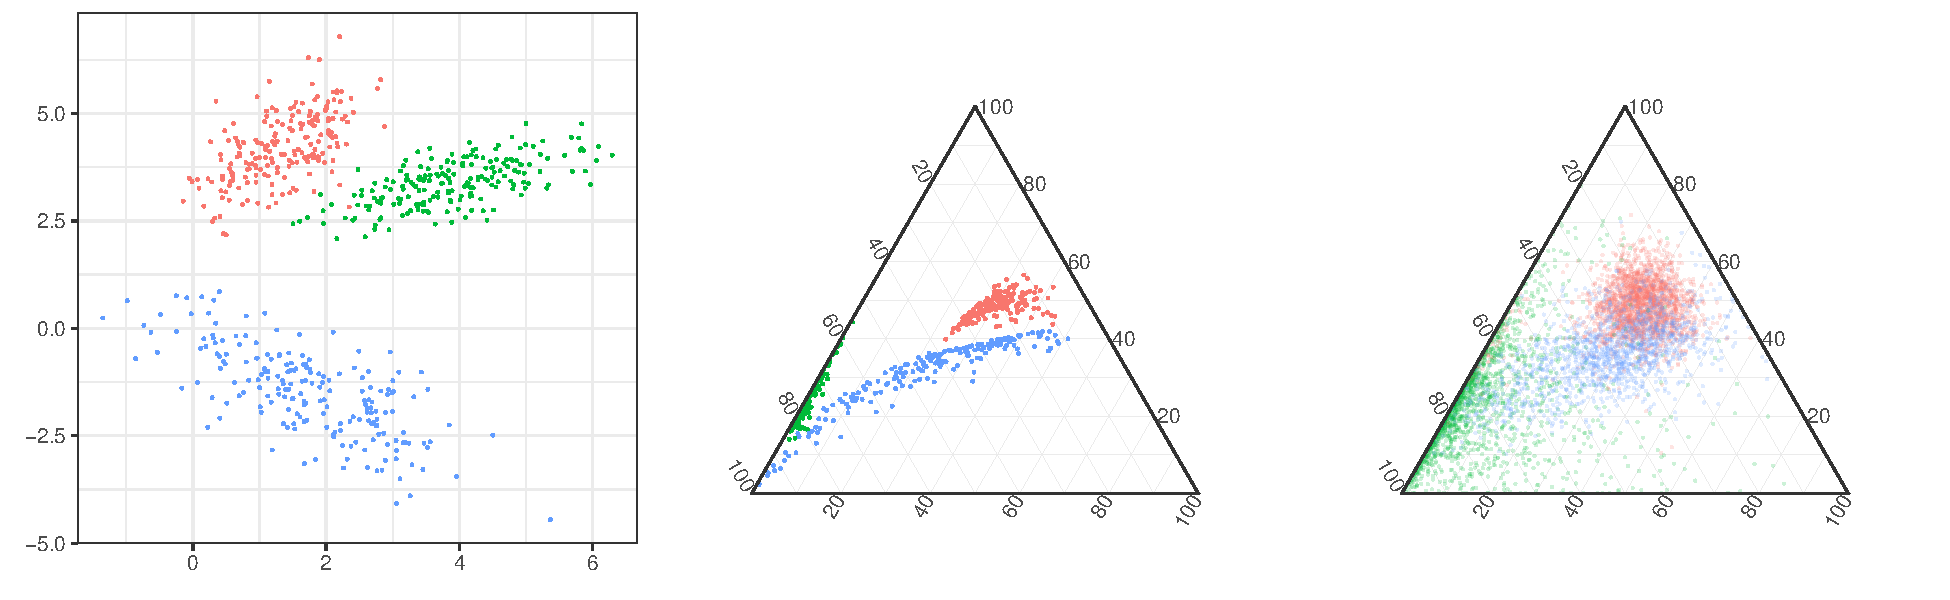
\includegraphics[width = \textwidth]{plots/simulated_reg}
\end{figure}

The fully specified model is extremely inefficient. As $S$ increases, the dimensionality of
    $\bm{\theta}$ increases linearly, which renders it inappropriate for modelling the SLOSH data.  
    However, we can consider other transformations of the data to keep the dimensionality of 
    $\bm{\theta}$ at an appropriate level.
    In the SLOSH data, let $\bm{x}_{is}$, the covariates associated with observation $i$ at location $s$,
    consist of $\bm{x}_{i,\text{obs}}$, the (scaled) parameters under which the $i$th storm is modelled,
    along with $\bm{x}_{s,\text{loc}}$, information pertaining to the $s$th location such as (scaled) 
    latitude and longitude, and $\bm{x}_{is,\text{int}}$, any interaction thereof.  
    We consider a single interaction term describing the distance between the location of the storm eye 
    at landfall, and that of location $s$, in hectomiles. This results in a $\bm{\theta}$ of dimension 
    $5 + 2 + 1 = 8$.  Then we may add an additional fixed effect by location, $\varepsilon_s$.  Thus for 
    analysis of the SLOSH data we formulate the regression model as
    \begin{equation}
        \label{eqn:regressionmodelredux}
        \bm{y}_i \sim 
            \mathcal{PG}\left(\bm{y}\mid g(\bm{x}_i^T\bm{\theta}_i + \bm{\varepsilon}), \bm{1}\right)
            \;\hspace{1cm}\;
            \varepsilon_s \sim \mathcal{N}(\varepsilon \mid 0, \sigma_{\varepsilon}^2)
    \end{equation}
    where $\bm{x}_i$ has been overloaded as discussed.  


    
